%-----------------------------------LICENSE------------------------------------%
%   This file is part of tikz_figures.                                         %
%                                                                              %
%   tikz_figures is free software: you can redistribute it and/or              %
%   modify it it under the terms of the GNU General Public License as          %
%   published by the Free Software Foundation, either version 3 of the         %
%   License, or (at your option) any later version.                            %
%                                                                              %
%   tikz_figures is distributed in the hope that it will be useful,            %
%   but WITHOUT ANY WARRANTY; without even the implied warranty of             %
%   MERCHANTABILITY or FITNESS FOR A PARTICULAR PURPOSE.  See the              %
%   GNU General Public License for more details.                               %
%                                                                              %
%   You should have received a copy of the GNU General Public License along    %
%   with tikz_figures.  If not, see <https://www.gnu.org/licenses/>.           %
%------------------------------------------------------------------------------%

% Use the standalone class for displaying the tikz image on a small PDF.
\documentclass[crop, tikz]{standalone}

% Import the tikz package to use for the drawing.
\usepackage{tikz}

% Needed for \mathbb command.
\usepackage{amssymb}

% Begin the document.
\begin{document}

    % Draw the figure.
    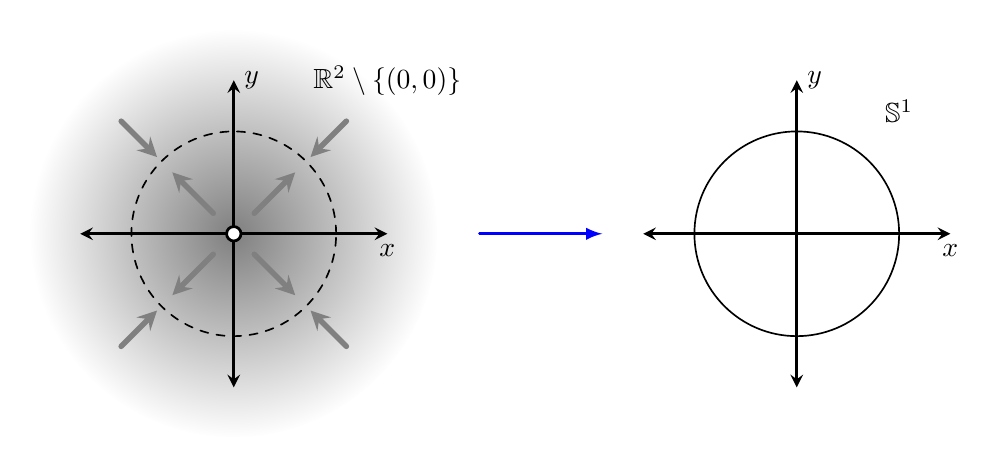
\begin{tikzpicture}[%
        scale = 1.3,
        line width = 1pt,
        line cap = round,
        > = stealth,
        every edge/.style = {%
            draw = black,
            very thick
        },
        grayarrow/.style = {%
            > = stealth,
            fill = gray,
            draw = gray,
            line width = 0.7mm,
            ->
        }
    ]

        % Gray gradient to represent the plane.
        \filldraw[%
            inner color = gray,
            outer color = white,
            draw = white
        ] (0.0, 0.0) circle (2);

        % Draw axes.
        \draw[<->] (-1.5, 0.0) to (1.5, 0.0) node [below] {$x$};
        \draw[<->] (0.0, -1.5) to (0.0, 1.5) node [right] {$y$};
        \draw[<->] (4.0, 0.0) to (7.0, 0.0) node [below] {$x$};
        \draw[<->] (5.5, -1.5) to (5.5, 1.5) node [right] {$y$};

        % Draw gray arrows indicating homotopy equivalence.
        \begin{scope}[every edge/.style = grayarrow]
            \draw (1.1, 1.1) edge (0.75, 0.75);
            \draw (-1.1, -1.1) edge (-0.75, -0.75);
            \draw (1.1, -1.1) edge (0.75, -0.75);
            \draw (-1.1, 1.1) edge (-0.75, 0.75);
            \draw (0.2, 0.2) edge (0.6, 0.6);
            \draw (-0.2, -0.2) edge (-0.6, -0.6);
            \draw (0.2, -0.2) edge (0.6, -0.6);
            \draw (-0.2, 0.2) edge (-0.6, 0.6);
        \end{scope}

        % Dotted line for the circle, the image of the homotopy.
        \draw[%
            dashed,
            draw = black,
            semithick
        ] (0.0, 0.0) circle (1);

        % Add a puncture at the origin.
        \filldraw[fill = white, draw = black] (0.0, 0.0) circle (2pt);

        % Blue arrow connecting the figures.
        \draw[> = latex, draw = blue, ->] (2.4, 0.0) to (3.6, 0.0);

        % Draw the unit circle.
        \draw[draw = black, semithick] (5.5, 0.0) circle (1);

        % Label the plane and the circle.
        \node at (1.5, 1.5) {$\mathbb{R}^{2}\setminus\{(0,0)\}$};
        \node at (6.5, 1.2) {$\mathbb{S}^{1}$};
    \end{tikzpicture}
\end{document}
